\begin{document}
\maketitle

\begin{abstract}
\noindent I ask what the complete wiring diagram of a fruit fly's brain knows about meeting another fly. To find out, I run a published simulation of that diagram as the brain of a fly in Minecraft, first on its own, then with one internal state switched on, then with a learning rule. I try hard to break every result. Run this way, I argue, the wiring knows how to react but not what it wants. The senses send mostly ``no'' or nothing to the neurons that decide whether to accept a male or fight, but keeping the female's two ``virgin'' neurons firing wakes her acceptance neurons. Keeping hunger neurons firing does no more than keeping an unrelated group firing. A memory forms once I supply the teaching signal that the model's taste neurons fail to send, and the fly hardly ever uses it. Along the way I found that most smells leave the model firing on its own for as long as I watched, and that several things I first believed were wrong.
\end{abstract}

\medskip
\noindent\textbf{Keywords:} connectome, \emph{Drosophila}, whole-brain simulation, innate behaviour, courtship, Minecraft

% ══════════════════════════════════════════════════════════════════════════════
\section{Introduction}
\label{sec:introduction}

Fruit-fly geneticists name a gene after what goes wrong when it breaks. A fly with a broken \emph{dunce} gene cannot learn that a smell comes with an electric shock \citep{dudai1976dunce}. A male with a broken \emph{fruitless} gene courts other males \citep{ryner1996control}. Behind the jokey names is the idea that much of what a fly does comes built in. Reared alone, a male courts the first virgin female he meets, and does it properly \citep{siegel1979conditioned}. He follows her, taps her with a foreleg to taste her, stretches out one wing and vibrates it to sing, and tries to mate. She decides. A virgin slows down and lets him. A female who has mated recently walks off, kicks, and holds out her ovipositor, the tube at the tip of her abdomen that she lays eggs through, until he gives up \citep{greenspan2000courtship}.

But built into what? A behaviour that nobody taught could live in two quite different places. It could be in the wiring, in which neuron connects to which, the way the ring of a doorbell lives in the circuit between the button and the bell. Or it could need the fly to be in a particular state, virgin or mated, hungry or fed. And some social behaviour is learned: a male who has spent an hour being turned down by a mated female courts half-heartedly for hours afterwards \citep{siegel1979conditioned}. In a living fly the three cannot be pulled apart, because every fly that has wiring also has states and a past.

A simulation can pull them apart. In 2024 the FlyWire consortium published the wiring diagram of a whole female fly brain, 139{,}255 neurons and about fifty million synapses \citep{dorkenwald2024neuronal}. A male followed in September 2026, with the nerve cord that runs his legs and wings \citep{berg2026sexual}. \citet{shiu2024drosophila} had already turned the female diagram into a simulation with one model neuron for every real one, and found that it does some of what flies do. A simulation like that is a fly with wiring and nothing else. It has no hormones or moods, and it has never learned anything. Whatever it does, the wiring can do alone. Whatever it cannot do needs something else, and I can add the something else back one piece at a time.

Forty years after the first complete wiring diagram, of a worm with 302 neurons \citep{white1986structure}, biologists still argue about how much of the worm's behaviour it explains. Much of the worm runs on chemistry, which a diagram does not show \citep{bargmann2013connectome}. Diagrams of bigger brains now cost a great deal \citep{microns2025functional}, so it is worth asking what a complete one knows on its own.

So I gave the simulated brain a body in Minecraft (\Cref{fig:overview}) and put two flies in a box.

\subsection{The Argument in Brief}
\label{sec:brief}

\emph{First}, the wiring alone carries reflexes. The simulated fly works her mouthparts on sugar and extends her ovipositor when her head is touched, and a randomly rewired brain does neither. \emph{Second}, it carries none of the decisions. The neurons with which a female accepts a male or fights another female can fire, but the senses tell them no, or nothing. A few of the male's courtship neurons do fire, mostly to the smell of another male. \emph{Third}, keeping her two ``virgin'' neurons firing wakes her acceptance neurons. Keeping the hunger and fullness neurons firing does no more than keeping an unrelated group firing, and real flies carry those states mostly in chemicals. \emph{Fourth}, once I supply the teaching signal that taste fails to deliver, the fly learns which smell came with sugar and does nothing with it. \emph{Fifth}, two flies in a box do not steer towards each other. So in this model ``built in or learned?'' has at least four answers: wiring, states carried by wires, states carried by chemicals, and learning. The diagram carries the first two, once someone switches the state on.

\subsection{Contributions}

I make four contributions.

\begin{enumerate}[leftmargin=*]
  \item A body in Minecraft for the published whole-brain fly model, and a male brain built the same way (\Cref{sec:experiment}).
  \item A map of which social behaviours this model produces from wiring alone, which need one internal state and which it cannot produce (\Cref{sec:reflexes,sec:absent,sec:states,sec:memory,sec:arena}).
  \item Two findings about the model itself. Its published smell centre cannot tell smells apart (\Cref{sec:experiment}), and most smells leave the model firing on its own after they have gone (\Cref{sec:absent}).
  \item A record of trying to break all of this, which overturned several of my own first claims (\Cref{sec:breaking}).
\end{enumerate}

\subsection{What This Paper Is Not}

It is not a claim that the model is a fly. A wiring diagram is to a brain roughly what a road map is to traffic: it shows every road and junction, but not which roads are busy or where anyone wants to go. The model adds some of the simplest traffic rules anyone has proposed, so when the simulated fly fails, the fault may lie in those rules, and I try to say when. Nor is it a new brain model. I rebuilt Shiu et al.'s and changed two things, both reversible (\Cref{sec:experiment}). Everything here happens in a computer, and testing its predictions (\Cref{sec:refutation}) is work for people with flies.

\subsection{Author Position}

I am an independent researcher. My earlier papers are about evaluating AI systems \citep{lijo2026compound,lijo2026pifbench,lijo2026niche,lijo2026tsb,lijo2026spirits}, and I have no training in biology. This paper does the same job on a different system: it puts a published model through tests, most with pass marks fixed in advance, and reports where it fails. An AI coding assistant helped to write the simulator, the Minecraft body, the analysis scripts and drafts of this text. Other copies of it then checked the claims against the result files (\Cref{sec:breaking}). Those copies share its blind spots, and nobody outside the project has checked the work yet.

This paper reads differently from my others because, unlike them, it was fun to do. I wanted to see what a fly's brain would do if I let it loose in Minecraft. So I have written it the way I would tell it, in the manner of Bill Capra's \emph{The Metaphysics of Farts} \citep{capra2022metaphysics}, a short essay that treats a silly subject with a straight face. The tests are as strict as in my other papers.

\subsection{Roadmap}

\Cref{sec:guide} is a guide for readers without biology and \Cref{sec:experiment} describes the experiment. \Cref{sec:reflexes,sec:absent,sec:states,sec:memory,sec:arena} give the results, \Cref{sec:breaking} tries to break them, and the last sections answer objections and list what would prove me wrong. The numbered notes hold the numbers. The story does not need them.

% ══════════════════════════════════════════════════════════════════════════════
\section{A Fly Brain for Readers Without Biology}
\label{sec:guide}

Nothing in the main text needs more biology than this section.

\subsection*{Neurons and spikes}

A neuron is a cell that passes on messages as tiny electrical pulses called spikes. How busy a neuron is gets counted in spikes per second, written Hz. A neuron at rest fires 0\,Hz, a busy one 50 or 100. To \emph{drive} a neuron is to make it fire. Where one neuron meets the next there is a synapse. A spike arriving at an excitatory synapse nudges the next neuron towards firing, and one arriving at an inhibitory synapse nudges it away. Which kind a neuron makes depends mostly on the chemical it releases, its neurotransmitter. For most neurons nobody has measured that chemical. The model uses a guess made by a computer program (a classifier) from microscope pictures, and makes each neuron all ``go'' or all ``stop''. That is the neuron's sign. Some neurons also pass current through direct contacts, called electrical synapses. The model has none.

\subsection*{The wiring diagram}

A fruit fly's brain has about 140{,}000 neurons (a human brain has about 600{,}000 times as many). A wiring diagram, or connectome, lists which neuron connects to which, and through how many synapses. It records nothing about what travels along the wires.

\subsection*{Three kinds of neuron}

Sensory neurons turn the world into spikes: smell receptors on the antennae, taste neurons on the mouthparts and legs, bristles that fire when they are bent, and an ear in the antenna. Descending neurons, about 1{,}300 of them, carry commands down the neck to the legs and wings. Everything in between, over a hundred thousand neurons, is where any deciding has to happen. \Cref{tab:cast} lists the neurons this paper mentions and the names I use for them.

\subsection*{States and chemistry}

A fly can be hungry or fed, virgin or mated. Part of that is carried by particular neurons that keep firing steadily. The virgin neurons, for example, fire until the female mates. Part is carried by chemicals such as hormones and neuropeptides (small protein messengers), released into the brain to change how other neurons respond. Biologists call this neuromodulation \citep{marder2012neuromodulation}. A wiring diagram can show the first kind but not the second.

\subsection*{Learning}

A fly learns which smells go with food in a part of its brain called the mushroom body. A smell switches on a small set of its cells, and if a dopamine ``teacher'' neuron fires at the same moment, the connections from those cells to the mushroom body's output neurons weaken. The next time the smell arrives, the output neurons hear it more faintly. That weakening is the memory. The output neurons push the fly towards or away from things.

\subsection*{Three technical words}

A \emph{seed} fixes the program's random numbers, such as when each stimulated neuron fires. Running several seeds is like testing the same fly again with fresh luck, so it shows how much a number wobbles by chance. The \emph{gain} turns every synapse in the brain up or down together. A gain of 1 is the published strength, and 1.4 makes each synapse 40 per cent stronger. A result that appears at only one exact gain is a coincidence of the numbers. A \emph{rewired} brain is the same brain with its connections shuffled at random, each neuron keeping its number of connections. A behaviour that survives rewiring cannot be due to the particular wiring alone.

\begin{table}[tbp]
\centering
\small
\renewcommand{\arraystretch}{1.1}
\begin{tabularx}{\textwidth}{@{}>{\RaggedRight}p{3.3cm}>{\RaggedRight}p{3.2cm}>{\RaggedRight\arraybackslash}X@{}}
\toprule
\textbf{Neurons} & \textbf{Nickname here} & \textbf{What they do in a real fly} \\
\midrule
MN9 & the licking neuron & swings the mouthparts out to feed \citep{shiu2024drosophila} \\
Giant fibre (DNp01) & the escape neuron & fires the escape jump \citep{vonreyn2014spike} \\
aBN1 & the grooming neuron & starts antennal grooming \citep{hampel2015neural} \\
DNa01, DNa02 & the steering neurons & turn a walking fly left or right \citep{rayshubskiy2025neural} \\
MDN & the moonwalker & walks the fly backwards \citep{bidaye2014neuronal} \\
DNp13 & the ovipositor neuron & extends the ovipositor, which a virgin does to accept a male and a mated female to refuse one \citep{mezzera2020ovipositor} \\
Or67d neurons & the pheromone detector & smell cVA, a scent males make that other flies react to \citep{kurtovic2007single} \\
SAG & the virgin neurons & active in virgins, turned down by mating \citep{feng2014ascending} \\
pC1a--c; pC1d/e, aIPg & the female's deciders: acceptance neurons; aggression deciders & set how receptive, or how aggressive, she is \citep{wang2021neural,deutsch2020neural,schretter2020cell} \\
vpoEN & the song relay & carry the male's song to the yes neuron \citep{wang2021neural} \\
vpoDN (DNp37) & the yes neuron & opens the genital plate to accept a male \citep{wang2021neural} \\
oviDN & the egg-laying neurons & start egg-laying \citep{wang2020neural} \\
P1; pIP10 & courtship neurons (his deciders); song command & start a male's courtship; send his song command to the wing \citep{vonphilipsborn2011neuronal,kohatsu2011female} \\
IPC (insulin), DH44, NPF, SIFa, AstA & hunger and fullness neurons & signal whether the fly has fed, largely by releasing neuropeptides \citep{pool2014feeding} \\
PAM, PPL1; MBONs & the teachers; the memory's outputs & reward and punishment signals to the mushroom body; its output neurons \citep{aso2014neuronal} \\
\bottomrule
\end{tabularx}
\caption{The cast: the neurons that appear in this paper, the nicknames I use for them, and what experiments on real flies have found them to do.}
\label{tab:cast}
\end{table}

% ══════════════════════════════════════════════════════════════════════════════
\section{The Experiment}
\label{sec:experiment}

Shiu et al.'s model treats every neuron as a leaky bucket. Each spike from a neighbour pours in a fixed cupful for every synapse between them, or scoops one out if the neighbour is inhibitory. The bucket leaks, and when the water rises 7 millivolts above its resting level it overflows: the neuron fires and empties. Nothing is tuned to make the fly behave. At full numerical precision my rebuild matches a transcription of their code spike for spike. At the lower precision I use for speed, a neuron on the brink of overflowing can tip the other way. In one of three test runs the difference then spreads to about a fifth of the spikes, though their total changes by under 1 per cent \note{1}.

Twenty times a second the Minecraft body turns what the fly smells, tastes and touches into firing of its own sensory neurons, and its own descending neurons move the body (\Cref{fig:overview}). Flowers smell of fruit or vinegar. Another fly smells of fly, and a male also of cVA, his pheromone, a scent one fly makes to signal to others. Bumping into anything fires every bristle on the head. The female map stops at the neck, so she walks on her steering neurons: the harder they fire the faster she goes, and when one side fires harder she turns that way. Nothing in the body says ``if touched, back away''. If the fly backs away, its moonwalker neurons fired. The flies are in effect blind. Light makes their eyes fire, but the eye's first relay neurons signal partly by being turned down, which a model neuron at rest cannot pass on. I built a male brain the same way from the male map.

Most of the numbers come from the bench, without Minecraft. I make one set of sensory neurons fire, usually 100 times a second for a second, and count what fires elsewhere. A louder sound or a harder touch means a higher rate.

\begin{figure}[tbp]
\centering
\begin{tikzpicture}[
  font=\footnotesize,
  box/.style={draw=black!55, rounded corners=3pt, align=center, inner sep=4pt, minimum height=2.3cm, text width=#1},
  arr/.style={-{Stealth[length=2mm]}, semithick, black!70},
  lab/.style={font=\scriptsize, text=black!70, above=1pt},
  sw/.style={draw=black!45, rounded corners=2pt, align=center, inner sep=3pt, text width=3.7cm, minimum height=1.3cm, fill=yellow!9},
]
\node[box=2.45cm, fill=green!7] (world) {\textbf{The Minecraft world}\\[3pt] flowers that smell, sugar and bitter blocks, walls, and another fly};
\node[box=2.35cm, fill=orange!9, right=0.8cm of world] (sense) {\textbf{Sensory neurons}\\[3pt] smell, taste, touch and the ear in the antenna};
\node[box=2.9cm, fill=blue!6, right=0.8cm of sense] (brain) {\textbf{The wiring diagram, running}\\[3pt] one model neuron for each real one; nothing tuned to behaviour};
\node[box=2.45cm, fill=red!6, right=0.8cm of brain] (dn) {\textbf{Descending and motor neurons}\\[3pt] steer, walk, walk backwards, jump, lick, sing};
\draw[arr] (world) -- node[lab]{senses} (sense);
\draw[arr] (sense) -- node[lab]{spikes} (brain);
\draw[arr] (brain) -- node[lab]{spikes} (dn);
\draw[arr] (dn.north) -- ++(0,0.42) -| node[pos=0.25, lab]{the body moves, so what it senses changes: one loop every 50\,ms} (world.north);
\node[sw, below=0.85cm of brain] (s2) {\textbf{2: + one state}\\ e.g.\ the fly's own ``virgin'' neurons kept firing};
\node[sw, left=0.25cm of s2] (s1) {\textbf{1: wiring only}\\ the diagram as published};
\node[sw, right=0.25cm of s2] (s3) {\textbf{3: + learning}\\ dopamine weakens the synapses of a memory};
\draw[arr] (s1.north) -- ($(brain.south west)!0.15!(brain.south east)$);
\draw[arr] (s2.north) -- (brain.south);
\draw[arr] (s3.north) -- ($(brain.south west)!0.85!(brain.south east)$);
\end{tikzpicture}
\caption{The experiment. A simulated fly brain, built neuron for neuron from a wiring diagram, runs a fly in Minecraft. The world is turned into firing of the fly's own sensory neurons, and the firing of its own descending neurons moves the body. The same brain runs in three settings that differ in nothing else.}
\label{fig:overview}
\end{figure}

A simulation always does something, so a behaviour counts as ``in the wiring'' only if it passes three tests fixed in advance. It must hold with every synapse turned down by 30 per cent and up by 40 per cent (gains 0.7 and 1.4). It must vanish when the brain is rewired at random. And it must hold in all fourteen versions of the female model (mine and thirteen alternatives to my own choices) and all thirteen of the male \note{2}.

A fly's smell centre has about fifty small knots of wiring (glomeruli), one for each type of smell receptor. A real smell sets off a few of them, like pressing a few keys on a piano. The first surprise was that in the published model any one key sounded the whole keyboard. Every smell set off the same two-thirds of the mushroom body, so every smell smelled the same. The culprit is about 150 local neurons that link the knots and that the model counts as excitatory. About half are of a kind whose pull in real flies is weak and passes largely through electrical synapses \citep{yaksi2010electrical}. Most of the rest are probably inhibitory neurons whose transmitter the classifier misread. I turned their output down to a quarter, the mildest cut I tried that keeps smells apart, and I use the measured transmitter wherever one is known \note{3}. In the female at the published synapse strength, only results that involve smell depend on these two changes. The one exception is sugar, which sets off the published smell centre in one run in five.

% ══════════════════════════════════════════════════════════════════════════════
\section{What the Wiring Does by Itself}
\label{sec:reflexes}

With the wiring alone the fly has five reflexes \note{4}, three of which Shiu et al.\ already found in this model: feeding on sugar, its suppression by bitter, and grooming. Two of the five pass every test set in advance. Sugar on the mouthparts makes the fly work them. Touch a female's head and she extends her ovipositor, even if the touch covers only a quarter of the bristles or one side of the head. Real females extend it to accept or refuse a male \citep{mezzera2020ovipositor}, but nobody has tested a touch on the head, so that one is a prediction. The other three each have a weak spot. Bitter nearly stops the feeding at the published strength but only slows it at gain 1.2 and above. The escape jump needs a loud sound, and at half the loudness it hardly fires. A strong push on the antenna makes the fly groom, though not at gain 0.7, and not once the weakest connections are removed.

Two behaviours I had counted as reflexes do not pass. Touch over most of a female's head turns down her steering neurons, which in the Minecraft body also set her walking speed, so a touched female stops. I call this the freeze, and no other sense causes it. But touching a tenth of the bristles speeds those neurons up instead. The freeze also fades as the weakest connections are removed, and is gone once every connection of fewer than five synapses is cut. When the male touches a female or tastes her with his legs, his moonwalker neurons fire and his courtship neurons stay silent, where a real male starts courting \citep{kohatsu2011female,clowney2015multimodal}. The backing also fails my tests. At gain 0.7 the touch and taste I usually test with no longer drive it. At 1.4 taste drives it less than half as hard. So I count it as a property of this model at its published strength.

Rewire the brain at random and every one of these reflexes disappears, though that test is blunt: almost nothing then gets from any sense to any descending neuron. A stricter rewiring keeps each connection within its broad class of neuron, such as sensory or descending. Under it a loud sound still fires the escape neuron at about 60 per cent of its normal rate, so that reflex needs only roughly the right kinds of connection. Touch sets off the escape, backing and steering neurons all at once, while the ovipositor neuron fires less than the average descending neuron \note{2}.

% ══════════════════════════════════════════════════════════════════════════════
\section{What the Wiring Does Not Do}
\label{sec:absent}

The neurons with which a female decides whether to accept a male or attack another female stay nearly silent whatever she senses. At gains from 0.7 to 1.4, at any stimulus rate and in all fourteen versions of the model, none fires more than two or three spikes a second. In the male the courtship neurons stay nearly silent on average too, but the smell of another male, cVA, makes a few of them fire. At the published strength one fires at about 6 spikes a second, and with a touch added five fire at up to 18. At gain 1.4 cVA alone makes 14 fire at up to 30. Real males court less when they smell cVA \citep{kurtovic2007single} but fight more \citep{wang2010identification}, and a weak push to courtship neurons of this kind starts a fight before it starts a song \citep{hoopfer2015p1}. So the male model either has the smell's effect backwards or is starting a fight, and these runs cannot tell which \note{5}.

The female's deciders can fire: drive the five kinds of neuron that feed each of them and every type in \Cref{fig:deciders}a fires. Every one sits one to three connections from every sense, so they are not cut off. What reaches them is mostly ``no'' or nothing (\Cref{fig:deciders}b). The male's pheromone pushes the aggression deciders further from firing, and touch lifts one pair of them halfway to firing while holding the song relay far below its firing point. The acceptance neurons receive almost nothing from any sense, and song, given as steady firing of the hearing neurons, barely reaches any of them.

Much of the ``no'' passes through six types of neuron that the classifier guessed to be inhibitory. Silencing them wakes no decider. If all six were in fact excitatory, the aggression deciders would answer the pheromone and the song relay would answer touch. At gain 1.4, touch would reach the yes neuron too. The acceptance neurons would still stay silent. In a real virgin they respond to the male's pheromone and song \citep{zhou2014central}, and a real male's courtship neurons respond to the touch of a female \citep{kohatsu2011female}. I count this as the model's most important miss.

\begin{figure}[tbp]
\centering
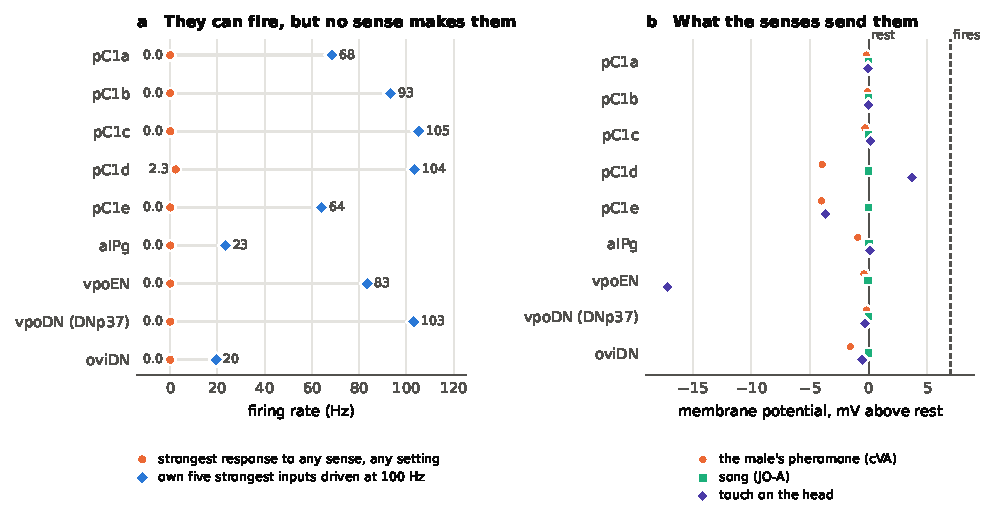
\includegraphics[width=\textwidth]{figures/fig_deciders.pdf}
\caption{The female's deciding neurons can fire, and the senses tell them no. \textbf{a}, the strongest rate each type of decider reaches to any sense in any setting (26 senses and combinations, synapse strengths 0.7--1.4, stimuli up to 300\,Hz, 14 versions of the model; 3 seeds each), against its rate when its own five strongest input types are driven at 100\,Hz. \textbf{b}, how full each decider's bucket gets under three senses at the published strength: its voltage in millivolts above rest (mean over its neurons and 3 seeds). A neuron fires at 7. Song here is steady firing of the ear's JO-A neurons.}
\label{fig:deciders}
\end{figure}

The model cannot start walking by itself either, though that is the most ordinary thing a fly does. In a clean box with nothing to smell but each other, two simulated females stood still for more than two minutes of brain time. Their eyes and noses fired, but not one descending neuron did. Part of this is the model's design: a model neuron has no activity of its own. Part is my smell-centre change, because under the published one the other fly's body odour sets them going (\Cref{sec:arena}). A real fly put in an empty dish soon walks about \citep{martin2004portrait}.

Most smells cause the opposite problem. A few seconds of the male's pheromone, a food odour or carbon dioxide leave about two thousand neurons firing on their own, the steering neurons among them. Twenty seconds after the smell had gone, when I stopped watching, they showed no sign of fading. I call this the self-sustaining state. Largely the same neurons fire whatever the smell. Touch, sound, sugar and the other fly's body odour alone leave nothing behind. The male's pheromone does the same in the male brain, and in the published models of both sexes the state takes in about eight thousand neurons. The state runs through the smell centre's excitatory local neurons. Turn them down to a tenth and it goes. Remove every connection from the brain back onto its own sensory neurons and it stays, so what keeps it going is in the brain itself \note{5}. In real flies the smell centre calms down soon after a smell ends \citep{wilson2004transformation}. The model's neurons never tire and its synapses never run down, so a loop of excitation, once lit, has nothing to put it out. But at a tenth most smells barely get through: only two of my ten test smells then set off more than a few dozen mushroom-body cells. So whether my version of the model keeps firing after a smell depends on how strong those local neurons really are, which nobody has measured.

Whichever rule I used to turn the transmitter guesses into ``go'' and ``stop'', the fly never steered clearly towards food. In my version, a food odour on one antenna turns her away. At gain 1.4 it still does in 11 of the 12 cases I tried. At 0.7 there is no turn to read, so like the backing this fails the synapse-strength test \note{5}.

% ══════════════════════════════════════════════════════════════════════════════
\section{What One State Adds}
\label{sec:states}

Keep the female's two virgin neurons firing and her acceptance neurons wake up \note{6}. Waking the acceptance neuron pC1a is no surprise, since the two virgin neurons supply nearly half its excitatory input. The signal also carries on one connection further, at every synapse strength I tried, to the yes neuron that opens her genital plate. Twenty random pairs of neurons with the same output strength (about as many synapses out) wake nothing. Nor do the virgin neurons in a rewired brain. This is half of the pathway traced in real flies \citep{wang2021neural}. A real virgin's yes neuron also needs the male's song, which reaches it through the song relay. In the model the relay stays silent even with song, and her deciders fire just as fast with or without the male's pheromone or song, so she says yes to nobody in particular. In the male I switched on the courtship neurons themselves, his deciders. They send his song command to the wing with nobody there to sing to, as they do in a real male on his own \citep{vonphilipsborn2011neuronal}. Twenty matched random sets of neurons do not, and nor do the courtship neurons in a rewired brain.

Keeping the hunger and fullness neurons firing, by contrast, changes no more than keeping an unrelated group firing. Partly that was bound to happen, since these neurons work mostly through neuropeptides, which the model lacks. In the female, the insulin (IPC) and DH44 neurons also have only about ten output synapses each. Her NPF, SIFa and AstA neurons have hundreds or thousands, but their paths to the feeding neurons are at most about a sixtieth as strong as sugar's, and two of the groups count as inhibitory here. So the states that work in this model are those whose neurons it treats as plain wires onto the deciders. That includes the virgin neurons, even though they are predicted to release serotonin, which acts as a neuromodulator in real flies.

The model also gets two things wrong. No state starts egg-laying. And at the model's standard settings a mated female (here, the brain with its virgin neurons left off) extends her ovipositor no more than a virgin, where a real one extends it more. Driving the virgin neurons three times as fast, or making every synapse 40 per cent stronger, makes the virgin's ovipositor neuron fire about a tenth less than the mated female's, which is the real direction.

% ══════════════════════════════════════════════════════════════════════════════
\section{What Learning Adds}
\label{sec:memory}

In the female model at its published strength, sugar and bitter tastes do not reach the dopamine teacher neurons. In real flies they do \citep{liu2012subset}, partly through octopamine, a neuromodulator whose chemical action the model lacks \citep{burke2012layered}. So I supplied the teaching signal myself whenever the fly tasted sugar, much as experimenters switch neurons on with light \note{7}, and the memory formed. After three pairings the smell that came with sugar reached the output neurons at about a tenth of its old strength, close to the lowest my rule allows. A second smell, given without sugar, kept about two-thirds. A teaching signal given just before the smell, or long after it, taught nothing. In one Minecraft run, on flowers that tasted of sugar, a weaker memory formed. In the male, whose map does not split sugar from bitter, taste as a whole does reach the punishment teachers. A smell paired with that taste then reaches the output neurons in those teachers' part of the mushroom body at half its old strength or less, with no help from me.

The fly did nothing with the memory. Where a before-and-after comparison exists, its walking and turning changed about as much as without the teaching signal. The route is there: driven hard, the memory's output neurons can turn the steering neurons on or off. But a smell drives them only weakly and reaches the steering neurons by other paths, so even silencing them barely changes what the legs receive. The memory is written in a notebook that is almost never opened. It could be opened more often if the neurons that the output neurons talk to sat closer to firing, as a fly's chemistry might keep them. With those neurons pushed to fire a few times a second, silencing the output neurons moved the left steering neurons by 3 to 7 spikes a second, against about 1 without the push. A memory can only quiet the output neurons, so silencing them is the most it could do, and I have not yet run a trained fly this way.

% ══════════════════════════════════════════════════════════════════════════════
\section{Two Flies in a Box}
\label{sec:arena}

The most entertaining results came from putting two flies in a box thirteen blocks across (\Cref{fig:arena}; \Cref{tab:arena}; Note~8). Every fly that walked in any box did so in the self-sustaining state, so the question is whether anything the flies sense steers them on top of it. Under the published smell centre the other fly's body odour starts the state. In that model the state drives the left steering neuron about nine times harder than the right, so two females circled to the left and never met. With my change, and a faint smell from flower patches that an earlier run had left by the wall, the females walked and bumped into each other by chance. Then they stayed together, because touch turned down their steering neurons. Real flies that bump into each other tend to move off \citep{ramdya2015mechanosensory}. These two stood pressed together for up to half a minute, extending their ovipositors at each other. A male and a female met far less often, and each meeting ended within seconds with the male walking backwards. In a properly cleaned box nothing moved, except that the male's pheromone set the female walking while he stood almost still until she touched him.

To get everyone moving I added a faint random input to every neuron, about one spike every five seconds, which I call the hum. Within a second or so it tips the brain into the self-sustaining state. On the hum, females met and stayed together, and males met females and backed out. On the bench, the touch of such a meeting drives his backing neurons most of the way on its own \note{4}. The male's song command never rose above the level the hum alone gives it, and neither did anyone's aggression neurons, except that a virgin female's reached about one spike a second on contact. Last, I ran two of the boxes again, three pairings in all, with new brain seeds and both flies let loose at the same moment, where before one had gone a few seconds ahead. The results held: two females on the hum met in every trial and on average spent almost half the time together, and a male and a female met briefly before he backed out. Then I switched off the females' sense of touch, which also took away their feel of the walls. They still met in every trial, but they no longer froze on contact, and the longest meeting fell from 16 seconds to under 4 (\Cref{tab:arena}; Note~8). So it is touch, through the freeze, that holds them together.

I measured whether a fly steers towards its partner before they first touch. In no box did it by more than a whisker, apart from the published model's steady left turn \note{9}. I first found a faint lean of the female towards the male, 24 recordings against 9. It came from her steady turn to the right and a male who happened to sit mostly on her right: with her own turning subtracted, 15 recordings lean towards him and 20 away. My flies are blind, and real males use sight to follow a female \citep{ribeiro2018visual}, so the box tests only whether the senses the flies have give them a reason to approach. A female whose virgin neurons I kept firing, on the hum with a male, makes the same point. Her yes neuron fired whether he was near or far, and her body logged nearly a hundred ``yes'' signals a minute, yet she did not steer towards him. Real virgins do not seek the male out either, but they slow down when he courts and open their genital plates when he sings \citep{bussell2014abdominal,wang2021neural}. Mine did neither in answer to him, apart from the stop that any touch causes.

\begin{figure}[tbp]
\centering
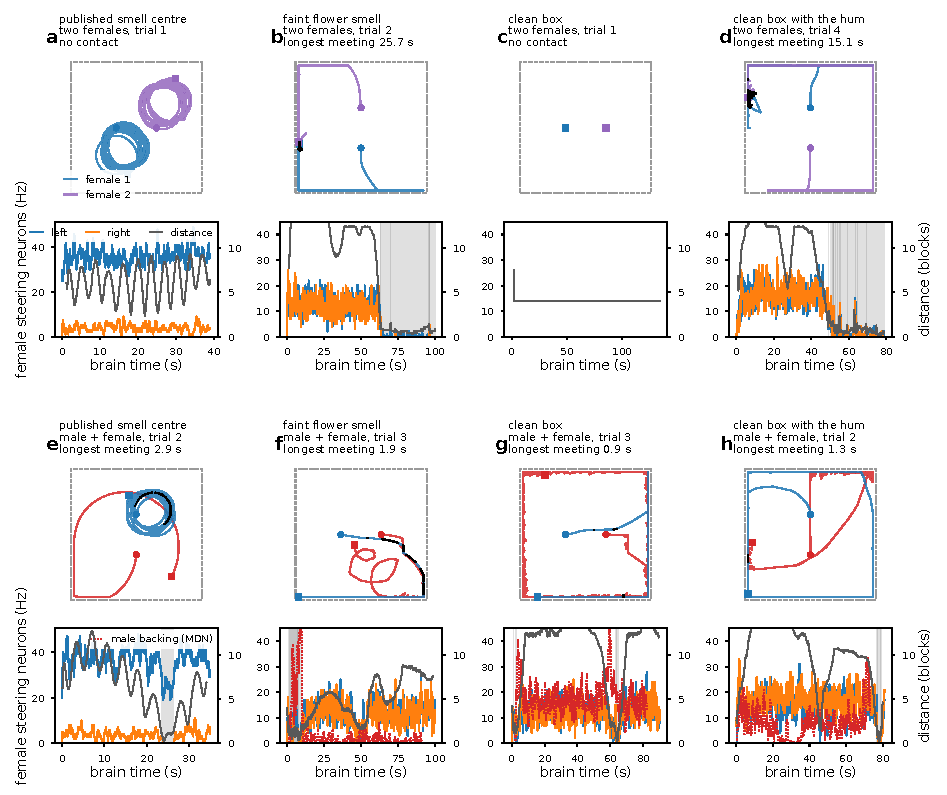
\includegraphics[width=\textwidth]{figures/fig3_print_encounters.pdf}
\caption{Two flies in a box, one trial for each box and pairing. \textbf{a--d}, two females; \textbf{e--h}, a male and a female, under the published smell centre (\textbf{a}, \textbf{e}), with my change and a faint flower smell at the wall (\textbf{b}, \textbf{f}), in a clean box (\textbf{c}, \textbf{g}) and in a clean box with the hum (\textbf{d}, \textbf{h}). Top: the paths walked (circle = start, square = end, black dots = contact, dashed = walls). Bottom: the female's left and right steering neurons, the distance between the flies (grey line), the male's backing neurons (red dotted) and contact (grey bands). Each panel shows the box's longest meeting (\textbf{a} and \textbf{c} had none), leaving out the two trials that began in contact because of the launch delay (Note 8).}
\label{fig:arena}
\end{figure}

% ══════════════════════════════════════════════════════════════════════════════
\section{Trying to Break It}
\label{sec:breaking}

I tried to break the results in three ways \note{10}. First, I re-ran the whole bench study from scratch, and all 124 result files it rewrote matched the previous run to the digit. Second, I had copies of the AI assistant check every sentence of a draft of this paper against the result files, and a further copy tried to argue away each problem that touched a main conclusion. Of 65 problems, 55 turned out to be real and 10 partly real. Most were wording that said more than the numbers do. A few were findings that did not survive, and the sections above say which. Third, I ran 60 new tests aimed at the claims (\Cref{tab:breaking}). For most I wrote the pass mark down before the run, and where a testing program repeats one of the paper's runs, I first made it reproduce the paper's result files to the digit.

\begin{table}[tbp]
\centering
\small
\renewcommand{\arraystretch}{1.12}
\begin{tabularx}{\textwidth}{@{}>{\RaggedRight}p{3.9cm}>{\RaggedRight}X>{\RaggedRight\arraybackslash}p{3.3cm}@{}}
\toprule
\textbf{Claim} & \textbf{How I tried to break it} & \textbf{What happened} \\
\midrule
The deciders are silent & every sense at gains 0.7--1.4 and at 200--300\,Hz, in all 14 model versions; their own inputs driven directly; the voltage and input of every decider; the inhibitory inputs silenced or flipped & holds in the female (at most 2--3\,Hz), not in the male, where cVA fires 1--14 of 148 courtship neurons (up to 30\,Hz), more with touch; mostly inhibition; with six guessed signs flipped the aggression deciders and song relay fire, the acceptance neurons still do not \\
The virgin state wakes them & gains 0.7--1.4; state rates 10--100\,Hz; 10 seeds; the hum; 20 random look-alike pairs; rewired brains & holds, but only half the real pathway \\
The courtship neurons send song & 20 random look-alike sets; the hum; one rewired brain & holds \\
Hunger does no more than an unrelated group & 10 seeds; the hum, in both sexes; added to the virgin state & holds (a 7\,Hz shift at 30\,Hz and 5 seeds shrank to 3\,Hz at 10 seeds; larger ones on the hum matched unrelated groups) \\
Reflexes are in the wiring & finer gains; stimulus rates 10--300\,Hz; a stricter rewiring & 2 hold throughout; 3 have a weak spot \\
The touched female freezes & weak connections removed (under 2 to 5 synapses); partial and one-sided touch; 5\,s of touch; other senses in place of touch & specific, but needs a strong touch and weak connections \\
The male backs away & gains; touch at 10--300\,Hz; what he smells; her touch, taste or smell removed & fails the gain test; touch gives most of it \\
The memory is learned & training in the wrong order; the teacher alone; other smells; longer training; two new seeds; a faster learning rule & holds \\
The memory is not used & its output neurons driven at up to 100\,Hz; a bypass of the smell route; the neurons they talk to kept close to firing & a route exists but is hardly used; with those neurons kept close to firing, silencing the output moves the steering neurons 3--7\,Hz \\
The model matches Shiu et al.'s & Shiu et al.'s code (in Brian2) on both versions of the model; time steps (the simulation's ticks) of 0.1--0.5\,ms; 3, 6 and 8 processor threads; new seeds & exact in full precision; smell runs drift apart; rates rise about 8\,\% at 0.5\,ms, because two timings round to the coarser tick \\
The model rests without input & smells, sugar, touch and sound for 3--10\,s, then silence; the smell centre's excitatory neurons turned down; the brain's connections onto its sensory neurons removed & fails after most smells; needs the smell centre's excitatory neurons \\
Nobody approaches & her own turning subtracted; his position shifted in time; each start counted once; new seeds & holds; the lean was not real \\
Touch keeps two females together & new seeds; their touch (of walls and of each other) switched off & holds (longest meeting 16\,s, under 4\,s without touch; no freeze on contact) \\
\bottomrule
\end{tabularx}
\caption{The tests aimed at each claim and what happened to it. Details in the notes and in \texttt{experiments/results\_edge/}.}
\label{tab:breaking}
\end{table}

% ══════════════════════════════════════════════════════════════════════════════
\section{Counterarguments}
\label{sec:counterarguments}

\subsection{``A Model This Simple Cannot Tell You Anything About a Real Fly''}

It cannot tell you what a real fly does. That needs a real fly. It can tell you what a complete wiring diagram contains when run with some of the simplest rules anyone has proposed. Some of what the model does, real flies do with the same neurons (feeding, grooming, the escape neuron, the first half of the virgin pathway). Some has no counterpart in a fly, such as a male backing away from a female he touches or tastes. So what the model does is a candidate for experiments, and what it cannot do points to candidates for what is missing.

\subsection{``Of Course a Model Without Hormones Cannot Be Hungry''}

Some of the negative results are unsurprising, and I have said which (\Cref{sec:states}). But the virgin state is partly chemical in real flies too, since sex peptide, a chemical the male passes on in mating, ends it \citep{feng2014ascending}. The state still works in the model because its last steps run on synapses. And a memory written entirely in synapses still hardly ever reaches the legs.

\subsection{``You Adjusted the Smell Centre Until It Did What You Wanted''}

I chose a quarter from four settings before I had written a test for it. Before a finer sweep I fixed a test in advance: different smells must set off largely different cells in the mushroom body. A quarter was still the mildest cut that passed it. At the published synapse strength, results that do not involve smell come out much the same either way, except that sugar sometimes sets off the published smell centre. The result that hangs most on the setting is the self-sustaining state, and with it the walking in the box. The state is larger without my change and absent at a tenth.

\subsection{``Five Trials Per Box Is Not Enough''}

For rates and proportions it is modest, and the notes give the spreads. Most of the arena claims are about presence or absence (no song command above what the hum alone gives, no steering towards the partner). Those need fewer trials, though what counts is the number of trials and not the number of moments recorded. Fifteen more trials with new seeds gave the same answers (\Cref{tab:arena}).

% ══════════════════════════════════════════════════════════════════════════════
\section{What Would Prove Me Wrong}
\label{sec:refutation}

Four things would defeat my argument.

\begin{enumerate}[leftmargin=*]
  \item A more faithful version of the same diagram would use measured transmitters or synapse strengths, or add electrical synapses. If one woke the female's acceptance neurons from the senses alone, or the male's courtship neurons from a female's touch or taste, the silence I found would belong to the simplified model. In real flies one pathway both excites and inhibits the male's courtship neurons \citep{clowney2015multimodal,kallman2015excitation}, a balance that a model in which every synapse pours the same cupful cannot set.
  \item Any reflex that disappears once predicted transmitters are replaced by measured ones along its path is not in the wiring. Of the behaviours here the freeze is the most fragile, since it rides on weak connections.
  \item If adding neuromodulation to the model, for example neuropeptide release from the hunger neurons, still left hunger doing nothing, then what is missing is not chemistry.
  \item If the self-sustaining state went out once the model's neurons were given a way to tire, that state would belong to the simplified neuron rather than to the wiring.
\end{enumerate}

The model also makes two predictions. A strong touch over most of a walking fly's head should quiet its steering neurons DNa01 and DNa02 while its ovipositor neuron fires, and a touch to a tenth of the bristles should not. And the fast drive from the head bristles to the ovipositor neuron should differ little between virgin and mated females. In the model it differs by about a tenth at most, so a large extra ovipositor extension in mated females would come from something slower, such as neuromodulation.

% ══════════════════════════════════════════════════════════════════════════════
\section{Limitations}
\label{sec:limitations}

The model has no neuromodulation, no electrical synapses, no development, no fatigue and no running down of synapses. Every neuron has the same leak and threshold, and the female model has no nerve cord. Dopamine, serotonin and octopamine, which act as neuromodulators in real flies, count here as ordinary excitatory synapses, and every neuron gets one sign, guessed by the classifier unless its transmitter is known. Sound arrives as steady firing, without the rhythm of real song. The male map does not split sugar from bitter taste, and I turned the male's synapses down so that his neurons get as much input on average as hers, which is a guess. Real flies start walking with descending neurons such as DNp09 \citep{bidaye2020two}, which answer no sense in this model, so I read walking from the steering neurons. The flies are blind. The arena is small, and one wiring diagram per sex cannot show how much real flies differ. Note 11 lists my other choices.

% ══════════════════════════════════════════════════════════════════════════════
\section{Conclusion}
\label{sec:conclusion}

A fruit fly's complete wiring diagram, set running with some of the simplest rules anyone has proposed, knows how to eat and how to hold out an ovipositor when touched. Less reliably, it knows how to jump at a loud noise and how to groom. Nobody had to put any of that in. It does not know what it wants. Its deciding neurons hear mostly ``no'' or nothing from the senses, and the female's acceptance neurons wake only once I keep her virgin neurons firing from outside. In a real fly that switch is set partly by chemistry, which is where I would look next, and where I would point anyone paying for the next map.

Two copies of my fly brain, mapped synapse by synapse, once stood in a clean white box for two minutes with only their eyes and noses working, like parked cars with the keys left in.

\bigskip
\noindent\emph{Solomon Shalom Lijo is an independent researcher.} \href{mailto:solomon@getromy.app}{\emph{solomon@getromy.app}}.

%%NOTES
